% This work is licensed under the Creative Commons
% Attribution-NonCommercial 3.0 Unported License. To view a copy of this
% license, visit http://creativecommons.org/licenses/by-nc/3.0/.

% This work is licensed under the Creative Commons
% Attribution-NonCommercial 3.0 Unported License. To view a copy of this
% license, visit http://creativecommons.org/licenses/by-nc/3.0/.

% ==========================================================================
%                     Festlegung der Dokumentenklasse
% ==========================================================================

% Dokumentklasse für Aufsätze, Berichte, etc.
\documentclass[paper=a4, german, titlepage]{scrartcl}

% Behebt ein paar Fehler in Latex
\usepackage{fixltx2e}

% ==========================================================================
%                            Detailtypographie
% ==========================================================================

\usepackage{microtype}

% ==========================================================================
%                             Zeichenkodierung
% ==========================================================================

% UTF-8 als Eingabe-Kodierung und T1 als Fontkodierung
\usepackage[utf8]{inputenc}
\usepackage[T1]{fontenc}

% ==========================================================================
%                               Schriftarten
% ==========================================================================

\usepackage{lmodern}

\setkomafont{disposition}{\normalfont\bfseries}

% ==========================================================================
%                           Spracheinstellungen
% ==========================================================================

% Deutsche Zeichenketten
\usepackage[german]{babel}


% ==========================================================================
%                        Bibliograhphie und Anhang
% ==========================================================================

\newcommand{\theappendix}{
  \clearpage
  \appendix
}

% Deutsche Guillemets mit \enquote{}
\usepackage[german=guillemets]{csquotes}

\usepackage[style=numeric-comp, backend=biber]{biblatex}
\bibliography{../literatur.bib}

% Nachnamen in Kapitälchen
\renewcommand*{\mkbibnamelast}[1]{\textsc{#1}}

% ==========================================================================
%                    Grafiken, Abbildungen und Tabellen
% ==========================================================================

% Verwenden von Farben und Grafiken
\usepackage{graphicx}
\usepackage{xcolor}

% Einbinden von ganzen PDF-Seiten
\usepackage{pdfpages}

% kleine Schrift für Bildunterschriften, Fettgedruckte Bildunterschriften
\usepackage[font=small,	labelfont=bf, format=plain]{caption}

% Für mehrere Objekte nebeneinander mit eigenen Bildunterschriften
\usepackage{subcaption}

% Beinhaltet \FloatBarrier , sodass nach diesem Befehl keine Floats mehr erscheinen
\usepackage[section]{placeins}

% Text umläuft Fließobjekte
%\usepackage{wrapfig}

% Tabellensatz
% \usepackage{tabularx}
\usepackage{booktabs}
\usepackage{longtable}

% Zum Verdrehen von Objekten. Nur mäßig verwenden.
% \usepackage{rotating}

% Setzen des Pfades für eingebundene Bilder
% \graphicspath{{figs/}{bilder/}}

% ==========================================================================
%                    Mathematikumgebungen und Einheiten
% ==========================================================================

% Paket für mathematische Umgebungen und Funktionen
\usepackage[intlimits]{amsmath}

% Zusätzliche Mathematische Schriftarten
\usepackage{amsfonts}

% Zusätzliche Mathematische Symbole
\usepackage{amssymb}

% Zum Setzen Kommutativer Diagramme
% \usepackage{amscd}

% Textsatz in der Matheumgebung
\usepackage{amstext}

% Aufrechte griechische Buchstaben
%\usepackage{upgreek}


% Diagramme mit tikz und Gnuplot zeichnen
% \usepackage{tikz}
% \usepackage{tikz-qtree}
% \usepackage{gnuplot-lua-tikz}

% ==========================================================================
%               automatischer Satz von Einheiten mit SIUnitX
% ==========================================================================

\usepackage[
% Stellt den Fehler separat dar: Siehe SIUnitX-Manual
  separate-uncertainty = true,
]{siunitx}

% Babel stellt SIUnitX auf deutsch ein, wenn german gewählt wird
\addto\extrasgerman{\sisetup{locale = DE}}

% Kürzen von Einheiten in SIUnitX ermöglichen
% \usepackage{cancel}

% ==========================================================================
%                  Aufzählungen, Referenzen und Links
% ==========================================================================

\usepackage{enumitem}

% Formattiert URLs, so dass sie sich z.B. besser vom Text abheben
\usepackage{url}

% TrueType-Schrift für URLs
% \urlstyle{tt}


% Verlinkungen innerhalb und außerhalb des PDF-Dokuments
\usepackage[colorlinks=false]{hyperref}

% intelligente Verlinkungen
\usepackage{cleveref}

% ==========================================================================
%                            Textsatzparameter
% ==========================================================================

% Vermeidung von "Schusterjungen" Höchstwert 10000, dann dürfen
% theoretisch keine Schusterjungen mehr auftreten.
\clubpenalty = 3000
% Vermeidkung von "Hurenkindern" Höchstwert 10000, dann dürfen
% theoretisch keine Hurenkinder mehr auftreten.  Es werden beide
% Einstellungen benötigt.
\widowpenalty = 3000
\displaywidowpenalty = 3000

\newcommand{\name}[1]{\textsc{#1}}
\renewcommand{\d}{\ensuremath{\mathrm{d}}}

\titlehead{{TU Dortmund \hfill WS~13/14\\}
Fakultät Physik\\
Fortgeschrittenenpraktikum}

\subject{Versuchsprotokoll}
\title{Der Helium-Neon-Laser}
\subtitle{Versuch 61}

\author{Daniel Meißner\\
{\normalsize\url{daniel.meissner@udo.edu}}
\and
Kevin Moch\\
{\normalsize\url{kevin.moch@udo.edu}}}

\date{5. März 2013}

\begin{document}
\maketitle

\tableofcontents
\clearpage

\section{Einleitung}
In diesem Versuch soll die Funktionsweise eines Helium-Neon-Lasers
verstanden werden. Dazu werden die Wellenlänge und die Polarisation 
des Laserlichtes untersucht, sowie zwei TEM-Moden vermessen und 
die Stabilität des Lasers überprüft.

% This work is licensed under the Creative Commons
% Attribution-NonCommercial 3.0 Unported License. To view a copy of this
% license, visit http://creativecommons.org/licenses/by-nc/3.0/.

\section{Theorie}

\begin{figure}
  \centering
  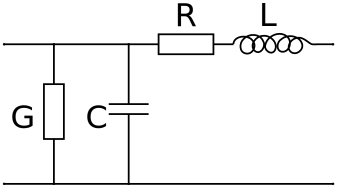
\includegraphics[scale=0.6]{ersatzschaltung}
  \caption{%
    Ersatzschaltung eines Koaxialkabels zwischen $x$ und $x + \d x$.
    Die Größen $R, L, G, C$ heißen Leitungskonstanten oder
    Leitungsbeläge.  Bei einer verlustfreien Leitung ist $R = G = 0$.
    Durch eine Betrachtung dieser Ersatzschaltung kann die
    Telegraphengleichung hergeleitet werden.}
  \label{fig:ersatz}
\end{figure}

Die Beschreibung der Ausbreitung von Signalen auf Leitungen ist
Gegenstand der Leitungstheorie.  Eine Leitung (zum Beispiel eine
Koaxialleitung, die in diesem Versuch verwendet wird) kann durch zwei
parallel verlaufende Leiter modelliert werden.  Grundaufgabe der
Leitungstheorie ist es, den zeitlichen Verlauf von Stromstärke $I(t, x)$
und Spannung $U(t, x)$ an jedem Ort $x$ der Leitung zu bestimmen.

Dazu wird ein Leitungstück von $x$ nach $x + \d x$ durch die
Ersatzschaltung aus Abbildung~\ref{fig:ersatz} dargestellt.  Die
Leitungsbeläge $R, L, G, C$ heißen auch Leitungskonstanten: $L$ und $C$
heißen Induktivitäts- bzw. Kapazitätsbelag, $R$ und $G$ heißen ohmscher
Belag bzw. Querleitfähigkeitsbelag.  Die beiden letzten kommen durch die
endliche Leitfähigkeit des Leitermaterials (Längsspannungsverluste) und
dielektrische Verlustströme zwischen der Isolierung der beiden Leiter
zustande.  Zwischen den Leitungsbelägen gibt es folgenden Zusammenhang:
%
\begin{equation}
  \label{eq:belagsformel}
  G = \frac{RC}{L}
\end{equation}

\subsection{Telegraphengleichung}

Im allgemeinen ergibt sich durch Betrachtung der Ersatzschaltung ein
System gekoppelter partieller Differentialgln. für $U$ und $I$.  Im
Falle konstanter Beläge kann dieses entkoppelt werden und es folgt eine
verallgemeinerte Wellengleichung:
%
\begin{equation}
  \label{eq:wellengl.}
  \pdn{2}{U}{x} - LC \pdn{2}{U}{t} = (LG+RC) \pd{U}{t} + RGU
\end{equation}
%
Diese Gleichung wird auch oft als Telegraphengleichung bezeichnet.  Die
Lösungen sind gedämpfte, hin- und rücklaufende harmonische Wellen:
%
\begin{equation}
  \label{eq:loesung}
  U(t, x) = U_0 \,e^{\iunt\omega t \pm \gamma x}
\end{equation}
%
Der Faktor $\gamma = \alpha + \iunt \beta = \sqrt{(R+\iunt \omega L)(G +
  \iunt \omega C)}$ heißt Ausbreitungskonstante, $\alpha$ heißt
Dämpfungsbelag und $\beta$ heißt Phasenbelag.  Die Phasengeschwindigkeit
der Welle ist daher frequenzabhängig und führt zu einer Verzerrung des
Signals.

\subsection{Leitungswellenwiderstand}

Die Art der Verzerrung wird vom Leitungswellenwiderstand beeinflußt,
welcher durch das Verhältnis von Strom- und Spannungswellen, die sich in
eine gemeinsame Richtung ausbreiten, bestimmt ist.  Für ein
sinusförmiges Signal mit der Frequenz $\omega$ ist der Wellenwiderstand
daher
%
\begin{equation}
  \label{eq:wellenwiderstand}
  Z_0 = \frac{U(\omega)}{I(\omega)} = \sqrt{\frac{R + \iunt \omega
      L}{G + \iunt \omega C}}\:.
\end{equation}
%

\subsection{Spannungs- und Strompulse}

In der Digital- und Nachrichtentechnik haben die Signale, die über eine
Leitung übertragen werden, oft die Form eines Pulses.  Die Lösungen der
entsprechenden Telegraphengleichung haben dann die Form eines hin- und
rücklaufenden Pulses, der durch die Reflexion am Leitungsende entsteht.
Der Quotient
%
\begin{equation}
  \Gamma = \frac{U_\text{r}}{U_0} = \frac{Z_\text{L} - Z_0}{Z_\text{L} + Z_0}
\end{equation}
%
heißt Reflexionsfaktor, wobei $Z_L$ hier die Lastimpedanz am Verbraucher
darstellt.  Mit seiner Hilfe kann die Form der rücklaufenden Welle aus
dem Eingangspuls berechnet werden.  Dazu wird die
\name{Laplace}-Transformation verwendet.  Sei nämlich $\tilde{U}_0(s)$
die \name{Laplace}-Transformierte der Spannung des einlaufenden und
$\tilde{U}_\text{r}(s)$ die \name{Laplace}-Transformierte der Spannung
des reflektierten Signals am Ort $x$ zur Zeit $t$, dann gilt
%
\begin{equation}
  \label{eq:reflex}
  \tilde{U}_\text{r}(s) = \Gamma\, \tilde{U}_0(s).
\end{equation}
%
Aus der Umkehrung dieser Formel unter Ausnutzung der inversen
\name{Laplace}-Transformation der zeitliche Verlauf der Spannung
$U_\text{r}(t, x)$ bestimmt werden.  Je nach Leitungsabschluß ergeben
sich hier verschiedene Signalformen.  Im Fall $Z_\text{L} = Z_0$ liegt
die sogenannte Leitungsanpassung vor, d.\,h. der Reflexionsfaktor
$\Gamma = 0$ und es gibt keine reflektierte Welle.

\subsection{Mehrfachreflexionen}

Ein Signal, das durch die Leitung läuft, wird nicht nur am Ende der
Leitung reflektiert, sondern auch am Anfang, wenn der Reflex wieder dort
ankommt.  So ergibt sich eine Reihe von Mehrfachreflexionen zwischen den
Kabelenden.  Bei jedem Reflex wird die Amplitude des Signals um einen
entsprechenden Reflexionsfaktor $\Gamma$ geschwächt.  Sei der
Reflexionsfaktor des Kabelanfangs $\Gamma_\text{a}$ und der des
Kabelendes $\Gamma_\text{e}$, dann gilt im Grenzfall unendlicher
Reflexion für die Amplitude der Signalspannung:
%
\begin{equation}
  U_\infty = U_0(1 + \Gamma_\text{e} + \Gamma_\text{a} \Gamma_\text{e}
  + \Gamma_\text{a} \Gamma_\text{e}^2 + \Gamma_\text{a}^2
  \Gamma_\text{e}^2 + \dotsb) = U_0 \:\frac{1 + \Gamma_\text{e}}{1
    - \Gamma_\text{a} \Gamma_\text{e}}
\end{equation}
%

Befinden sich im Kabel zusätzlich Störstellen (z.\,B. wenn zwei
verschiedene Kabel aneinander gesteckt sind), gibt es auch an diesen
Stellen Reflexionen.  Um den Überblick zu behalten, kann es in solchen
Fällen hilfreich sein, einen sogenannten Impulsfahrplan anzufertigen.
In Abschnitt~\ref{sec:durchfuehrung-mehrfachreflexion} wird eine
Situationen, in der zwei unterschiedliche Kabel verbunden sind,
beschrieben.

\subsection{Ausgewählte Leitungsabschlüsse}

In diesem Abschnitt werden die Signalverläufe zu drei verschiedenen
Abschlußwiderständen berechnet.  Die erhaltenen Funktionen werden später
verwendet, um eine Ausgleichsrechnung mit den aufgenommenen Meßwerten
durchzuführen.  Der einlaufende Signalverlauf\footnote{Die Amplitude
  wird hier auf 1 normiert, um die Rechnungen nicht zu überladen.  Da
  die \name{Laplace}-Transformation eine lineare Abbildung ist, kann ein
  Faktor für die Amplitude nachträglich hinzugefügt werden.}  kann mit
der \name{Heaviside}-Funktion~$\Theta$ so geschrieben werden:
%
\begin{equation}
  U_0(t) = \Theta(t).
\end{equation}
%
Die \name{Laplace}-Transformierte lautet dann $\tilde{U}_0(s) = s^{-1}$.
Mit Formel~\eqref{eq:reflex} wird daraus durch Rücktransformation der
Reflex am Leitungsende berechnet.

\paragraph{Abschluß durch Induktivität} Im Falle einer Induktivität als
Abschluß ist $Z_\text{L} = \iunt\omega L$ und damit ergibt sich für $s =
\iunt\omega$ der Reflexionsfaktor zu
%
\begin{equation}
  \Gamma = \frac{sL - Z_0}{sL + Z_0} = \frac{s - \tau^{-1}}{s + \tau^{-1}}
\end{equation}
%
mit $\tau := L/Z_0$. Jetzt wird gemäß Formel~\eqref{eq:reflex} das
reflektierte Signal berechnet.  Zerlege dazu $\Gamma \tilde{U}_0(s)$ in
Partialbrüche:
%
\begin{equation}
  \tilde{U}_\text{r}(s) = \Gamma\tilde{U}_0(s) = \frac{s - \tau^{-1}}{s(s
    + \tau^{-1})} = \frac{2}{s + \tau^{-1}} - \frac{1}{s}
\end{equation}
%
Nach den Eigenschaften der \name{Laplace}-Transformation bezüglich
Translation das reflektierte Signal für $t>0$ erhalten:
%
\begin{equation}
  \label{eq:ind_reflex}
  U_\text{r}(t) = 2e^{-\frac{t}{\tau}} - 1.
\end{equation}

\paragraph{Abschluß durch Induktivität und ohmschen Widerstand} In
diesem Fall wird $Z_\text{L} = R + \iunt \omega L$ und der
Reflexionsfaktor lautet
%
\begin{equation}
  \Gamma = \frac{R + sL - Z_0}{R + sL - Z_0} = \frac{s + (R-Z_0)L^{-1}}{s + \tau^{-1}}
\end{equation}
%
mit $\tau := L/(Z_0 + R)$.  Jetzt wird analog zu oben verfahren.  Eine
Partialbruchzerlegung von $\Gamma \tilde{U}_0(s)$ liefert:
%
\begin{equation}
  \tilde{U}_\text{r} (s) = \Gamma \tilde{U}_0(s) = \frac{s + (R -
    Z_0)L^{-1}}{s(s + \tau^{-1})} = \frac{\Gamma_0}{s} + \frac{1
    - \Gamma_0}{s + \tau^{-1}}
\end{equation}
%
mit $\Gamma_0 := \frac{R - Z_0}{R + Z_0}$.  Daraus wird das reflektierte
Signal durch Rücktransformation erhalten:
%
\begin{equation}
  \label{eq:ind_ohm_reflex}
  U_\text{r}(t) = \Gamma_0 + (1 - \Gamma_0) e^{-\frac{t}{\tau}}.
\end{equation}

\paragraph{Abschluß durch Kapazität und ohmschen Widerstand} Hier ist
$Z_\text{L} = R + \frac{1}{\iunt \omega C}$ und der Reflexionsfaktor
lautet dann:
%
\begin{equation}
  \Gamma = \frac{\frac{1}{sC} + R - Z_0}{\frac{1}{sC} + R + Z_0}
  = \frac{\Gamma_0 s + \tau^{-1}}{s + \tau^{-1}} 
\end{equation}
%
mit $\Gamma_0$ wie oben und $\tau := (R+Z_0) C$.  Nach der
Partialbruchzerlegung
%
\begin{equation}
  \Gamma \tilde{U}_0(s) = \frac{1}{s} + \frac{\Gamma_0 - 1}{s + \tau^{-1}}
\end{equation}
%
lautet nach Rücktransformation das reflektierte Signal so:
%
\begin{equation}
  \label{eq:cap_ohm_reflex}
  U_\text{r}(t) = 1 + (\Gamma_0 - 1) e^{-\frac{t}{\tau}}.
\end{equation}

% This work is licensed under the Creative Commons
% Attribution-NonCommercial 3.0 Unported License.  To view a copy of
% this license, visit http://creativecommons.org/licenses/by-nc/3.0/.

\section{Aufbau und Durchführung}

\subsection{Aufbau der Apparatur}

Zur Untersuchung der Trägheitsmomente wird in diesem Versuch eine
sogenannte Drillachse verwendet.  In \cref{fig:drillachse} ist eine
solche skizziert.  Sie besteht aus einer drehbar gelagerten Achse, die
über eine Spiralfeder an den Rahmen der Lagerung oszillatorisch
gekoppelt ist.  An der Spitze dieser Achse werden die zu untersuchenden
Körper befestigt.

Mithilfe dieser Apparatur können die eingespannten Körper nun zu
Schwingungen angeregt werden, über deren Periodendauer sich dann das
Trägheitsmoment derselben berechnen läßt.  Dabei muß beachtet werden,
daß in Formel~\eqref{eq:periode} das Gesamtträgheitsmoment steht.  Im
Falle dieser Versuchsanordnung setzt sich dieses aus dem
Eigenträgheitsmoment~$I_\text{D}$ der Drillachse und dem Trägheitsmoment
$I_\text{K}$ des zu untersuchenden Körpers zusammen.  Sind also
Richtgröße~$D$ und Eigenträgheitsmoment~$I_\text{D}$ der Apparatur
bekannt, so kann das Trägheitsmoment~$I_\text{K}$ gemäß
\begin{equation}
  \label{eq:traegheit-winkelricht-drill}
  I_\text{K} = \frac{D T^2}{4 \pi^2} - I_\text{D}
\end{equation}
bestimmt werden.

\subsection{Bestimmung der Winkelrichtgröße}

Zur Bestimmung der Winkelrichtgröße~$D$ wird ein dünner Stab an der
Drillachse so befestigt, daß die Drehachse durch den Schwerpunkt
verläuft.  Jetzt wird in einem Abstand~$r$ vom Drehpunkt eine Federwaage
am Stab eingehängt und um den Winkel~$\phi$ ausgelenkt.  Hierbei sollte
die Federwaage am besten senkrecht zum Stab und zur Rotationsachse
gehalten werden, da so der Betrag vom $\vec{M}$ einfach durch
\begin{equation}
  | \vec{M} | = | \vec{r} \times \vec{F} | = r F \sin \angle(\vec{r},
  \vec{F}) = r F
\end{equation}
bestimmt werden kann.  Die Winkelrichtgröße kann dann gemäß
Gleichung~\eqref{eq:drehmoment-winkelricht} so bestimmt werden:
\begin{equation}
  \label{eq:winkelricht-kraft-abstand-winkel}
  D = \frac{r F}{\phi}.
\end{equation}
Hierbei wird sowohl der Abstand als auch der Winkel variert, um eine
Meßreihe mit zehn Meßwerten zu erhalten.

\subsection{Bestimmung des Trägheitsmoments der Drillachse}

Das Trägheitsmoment der Drillachse wird ermittelt, indem eine nahezu
masselose Stange, mit der zwei Gewichte in gleichem Abstand~$a$ vom
Schwerpunkt starr verbunden sind, an der Drillachse befestigt wird.  Die
Trägheitsmomente der Gewichte sowie der Stange sind bekannt.  Das
beschriebene System wird nun für verschiedene Abstände~$a$ zu
Schwingungen angeregt und die Periodendauer~$T$ wird bestimmt.  Das
Gesamtträgheitsmoment in Formel~\eqref{eq:periode} setzt sich nun nach
Anwendung des \name{Steiner}schen Satzes für die beiden Gewichte so
zusammen:
\begin{equation}
  I = I_\text{D} + I_\text{S} + 2I_\text{G} + 2m_\text{G} a^2
\end{equation}
Hier bezeichnet $I_\text{S}$ das Trägheitsmoment der Stange und
$I_\text{G}$ dasjenige eines Gewichts bezogen auf einer zur Drehachse
parallen Achse durch den Schwerpunkt.  Da die verwendeten Gewichte
zylinderförmig sind und der Stab, an dem diese befestigt ist, lang und
dünn ist, ergibt sich schließlich für das Trägheitsmoment der Drillachse
aus Formel~\eqref{eq:periode}:
\begin{equation}
  \label{eq:traegheit-drillachse}
  I_\text{D} = \frac{D T^2}{4 \pi^2} - \frac{1}{12} m_\text{S} l^2 -
  m_\text{G} (R^2 - 2 a^2),
\end{equation}
wobei $l$ die Länge des verwendeten Stabes ist und $R$ der halbe
Durchmesser eines Zylinders.  Bei den angegeben Massen handelt es sich
jeweils um die Massen eines der Gewichte bzw. des Stabes.  Es wird eine
Meßreihe der Periodendauer für zehn verschiedene Abstände~$a$ des
Gewichts angefertigt.

\subsection{Untersuchung des Trägheitsmoments}


% This work is licensed under the Creative Commons
% Attribution-NonCommercial 3.0 Unported License. To view a copy of this
% license, visit http://creativecommons.org/licenses/by-nc/3.0/.

\section{Auswertung}

\subsection{Bestimmung des  effektiven Dämpfungswiderstands} Zur
Bestimmung des effektiven Dämpfungswiderstands werden aus
Abbildung~\fig{fig:thermodruck} die Minima und Maxima abgelesen. In
Tabelle~\fig{fig:minmax-thermo} finden sich diese Werte. Zur Bestimmung
des Exponenten in Gleichung~\eqref{eq:loesung} werden die Maxima und
Minima getrennt in eine Ausgleichsrechnung gegeben. Dies wird deshalb
gemacht, da in der Abbildung~\fig{fig:minmax-plot} zu erkennen ist, daß
die Punkte zu zwei verschiedenen Geraden gehören. Daher werden die
Minima und Maxima wie angekündigt getrennt durch eine Gerade
ausgeglichen und der Mittelwert der Steigungen bestimmt.


\subsection{Amplitudenverhältnisse bei Resonanzfrequenz}


% This work is licensed under the Creative Commons
% Attribution-NonCommercial 3.0 Unported License.  To view a copy of
% this license, visit http://creativecommons.org/licenses/by-nc/3.0/.

\section{Diskussion}
%
Zum Schluss sollen die Ergebnisse dieses Versuches diskutiert werden.
Die bestimmte Güte des Selektivverstärkers beträgt $Q=\num{118}$.  Am
Selektivverstärker wurde eine Güte von 100 eingestellt.  Die relative
Abweichung der beiden Werte beträgt \SI{18}{\percent}.  Es wurden in
diesem Versuch nicht direkt die Ausgangsspannungen bei den Frequenzen
gemessen, bei denen die Spannung auf $\frac{1}{\sqrt{2}}$ der
Höchstspannung gefallen ist, sodass relativ grobe Abschätzungen gemacht
werden mussten.  Außerdem ist es nicht möglich einen Fehler für die
bestimmte Güte anzugeben.  Es wird also festgestellt, dass der
verwendete Selektivverstärker tatsächlich die eingestellte Güte besitzt.

Bei der Bestimmung der Suszeptibilitäten der verwendeten Proben ergeben
sich nur geringe statistische Fehler.  Diese besitzen aufgrund der
geringen Messwerteanzahl nur eine schwache Aussagekraft und dürfen nicht
überschätzt werden. Die Werte für die Suszeptibilität der untersuchten
Proben, die sich bei den verschiedenen Verfahren ergeben, weichen
deutlich stärker voneinander ab als die errechneten statistischen Fehler
es angeben.

Um die Vorhersagen der Quantenmechanik auf ihre Genauigkeit zu
überprüfen sollen hier noch einmal die theoretischen Werte mit den
beiden experimentell bestimmten verglichen werden.  Die Ergebnisse sind
in \cref{tab:vergleich} zu sehen.

\begin{table}
  \centering
  \begin{tabular}{lSSSSS}
    \toprule
    & {$\chi_U$} & {$\chi_R$} & {$\chi$} &
    {$\frac{\chi_U-\chi}{\chi}$ in \si{\percent}} &
    {$\frac{\chi_R-\chi}{\chi}$ in \si{\percent}} \\
    \midrule
    Dy$_2$O$_3$ & 0.0234 &  0.0186 & 0.0251 &  6.8 & 25.9\\
    Nd$_2$O$_3$ & 0.0054 &  0.0039 & 0.0030 & 80.0 & 30.0\\
    Gd$_2$O$_3$ & 0.0130 &  0.0108 & 0.0136 &  4.4 & 20.6\\
    \bottomrule
  \end{tabular}
  \caption{Die experimentell bestimmten Werte im Vergleich mit den
    theoretischen Vorhersagen.  }
  \label{tab:vergleich}
\end{table}

Insgesamt werden die Vorhersagen gut bestätigt.  Die Größenordnungen
stimmen bei allen Messungen mit den Vorhersagen überein.  Die relativen
Fehler der Messung mit der Spannungsmethode sind außer beim
Neodymium(III)-oxid sehr gering.  Bei der Widerstandsmethode sind die
Fehler zwar insgesamt höher, dafür ist aber auch beim Neodym die
Abweichung geringer.

\FloatBarrier

% Literaturverzeichnis
\addcontentsline{toc}{section}{Literatur}
\printbibliography
% Anleitung auf jeden Fall zitieren
\nocite{v061}

\end{document}
